\chapter{Methodology}
\label{sec:problem}

% TODO: Page 38 of Improving Sequential Decision Making in Human-In-The-Loop Systems

% \begin{enumerate}
%     \item How to get transition and observation probabilities? Am I correct that these need to be given by Florian's model? How would this ever be known in the case of learning with real human drivers?
%     \item Is the Markov assumption satisfied even though the driver's attentiveness does not depend on the previous state and action?
%     \item What is known a priori?
%     \begin{itemize}
%         \item human's current action (assumption: no, for performance reasons)
%         \item reward function
%     \end{itemize}
% \end{enumerate}

\section{Lane keeping with a human in the loop as a POMDP}
\label{sec:lane_keeping_loop}

% TODO: Add state estimator + policy to agent? 
% See (POMDP definition) Planning and acting in partially observable stochastic domains)
\begin{figure}[ht]
    \centerfloat
    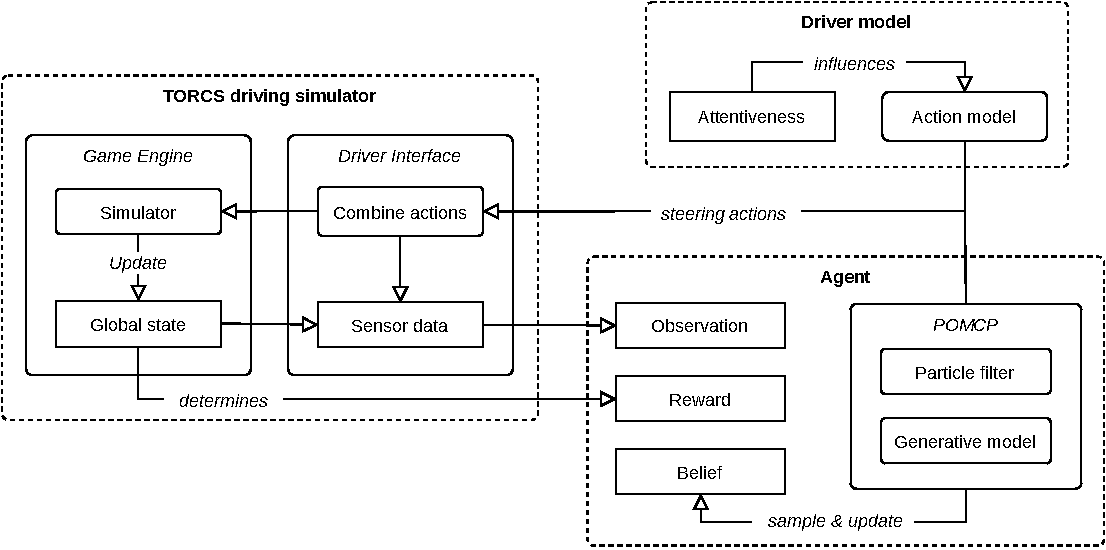
\includegraphics[width=1.2\linewidth]{figures/Components.pdf}
    \caption{Solution approach overview}
    \label{fig:overview}
\end{figure}

% TODO: Add: The agent can only recognize a state change of the driver after the driver has performed the first action in this state. This is because there are no observable clues about the duration of the driver's attentiveness and distraction.

\subsection{Driving simulator TORCS}

\subsubsection{State}
\label{sec:state}

% TODO: Define terminal state

The tracks will be round courses. Thus, there is no terminal state if everything goes well. If the car reaches an off-track position, however, the car is reset to be in the initial starting position again.\\

\begin{tabularx}{\textwidth}{@{}p{0.18\textwidth}>{\centering}p{0.22\textwidth}X@{}}
\toprule
\textbf{Name}           & \textbf{Measurement}          & \textbf{Description}                                           \\ \midrule

Gear \newline \textbf{(constant)} & \{$-1$, $0$, $1$,  \dots, $6$\} & Distance of the car from the start line along the track line. \textbf{Neither the human driver nor the agent can directly influence this with their actions.} \\ \midrule

RPM \newline \textbf{(constant)} & [0, $+\inf$) & Number of engine rotations per minute. \textbf{Neither the human driver nor the agent can directly influence this with their actions.} \\ \midrule

Speed \newline \textbf{(constant)}  & ($-\inf$, $+\inf$) (km/h) & Speed along the longitudinal axis of the car. \textbf{Neither the human driver nor the agent can directly influence this with their actions.} \\ \midrule

% Lift \newline \textbf{(constant)} & ($-\inf$, $+\inf$) (km/h) & Speed along the vertical axis of the car. Will be zero as we use completely flat terrain. \textbf{Neither the human driver nor the agent can directly influence this with their actions.} \\ \midrule

Side force & ($-\inf$, $+\inf$) (km/h) & Speed along the transverse axis of the car. This is directly influenced by the steering actions of both human driver and agent. \\ \midrule

Distance from start & [0, $+\inf$) (m) & Distance of the car from the start line along the track line. \\ \midrule

Angle          & [$-\pi$, $+\pi$] (rad) & Angle between car direction and track axis direction.  \\ \midrule

Lane position & ($-\inf$, $+\inf$)     & Horizontal distance between the car and the track axis. $0$ when the car is on the axis, $+1$ if the car is on the left edge of the track, and $-1$ if the car is on the right edge of the track. Greater numbers than $+1$ or smaller numbers than $-1$ indicate that the car is off-track. \\ \midrule

Driver attention & True / False & Whether the human driver is attentive or distracted.  \\ \bottomrule

\end{tabularx}

\subsubsection{Actions}
\label{sec:actions}

\begin{tabularx}{\textwidth}{@{}p{0.18\textwidth}>{\centering}p{0.22\textwidth}X@{}}
\toprule
\textbf{Name}           & \textbf{Measurement}          & \textbf{Description}\\ \midrule

\multicolumn{3}{@{}>{\centering}p{\linewidth}@{}}{\textit{In our simplified scenario, both the human driver and the agent can not accelerate, brake or switch gears.}} \\ \midrule

Steering         & [$-2$, $+2$] & The input to the car is generated by combining the agent's action with the human's steering action (see equation~\ref{eq:steering}). For the car,  $-1$ means full right (159 degrees) and $+1$ means full left (21 degrees). A value greater than +1 or lower than -1 can effectively reverse an opposite action of the human driver. \\ \bottomrule
\end{tabularx}\\\\

\noindent The human driver and the agent share control of the steering wheel. The speed of the car is fixed and cannot be altered; neither by human driver nor agent. The steering input of the driver $\mathcal{A}_{steer}^{driver}$ and agent $\mathcal{A}_{steer}^{agent}$ are combined to ${A}_{steer} \in [-1, +1]$ using equation~\ref{eq:steering}.

The agent needs to be able to fully counteract a distracted driver's actions. In the extreme case, while the car is in a curve, a distracted driver could steer into the opposite direction of the trajectory of the lane center. Thus, the car would not only diverge from the lane center but would even get off the road completely. The agent thus needs to reverse the driver's action in order to keep the car centered in the lane and follow the road curve. Therefore, we define the range for the agent's steering action as follows: $\mathcal{A}_{steer}^{agent} \in [-2, +2]$.

\begin{equation}
    \mathcal{A}_{\textrm{steer}} = \min(\, -1, \, \max(\, 1, \, (\mathcal{A}_{\textrm{steer}}^{\textrm{driver}} + \mathcal{A}_{\textrm{steer}}^{\textrm{agent}})\,)\,)
    \label{eq:steering}
\end{equation}

\subsubsection{Observations}
\label{sec:observations}

\begin{figure}[ht]
    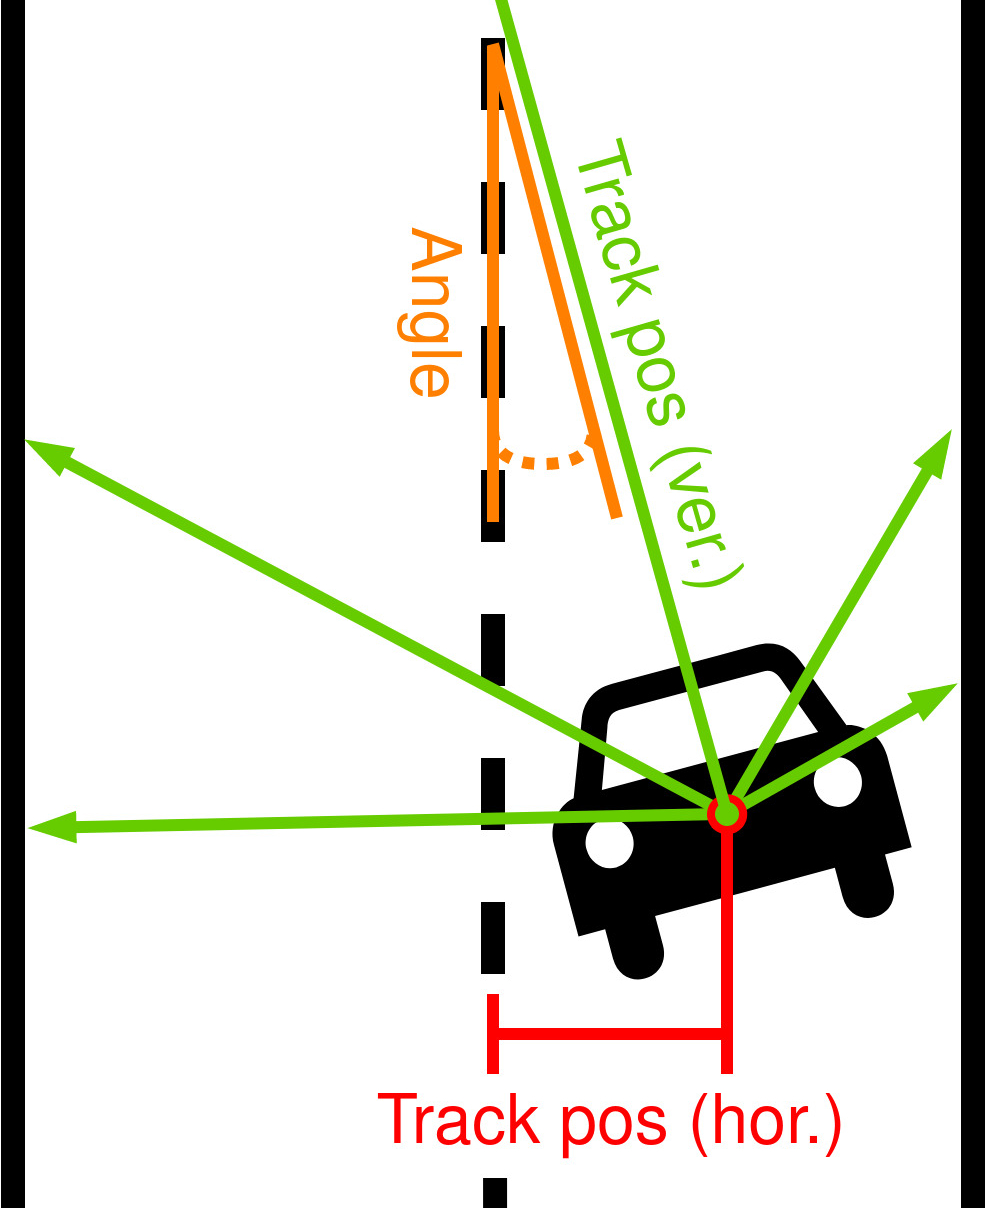
\includegraphics[width=0.3\linewidth]{figures/Observations.jpg}
    \centering
    \caption{Main environment observations}
    \label{fig:observations}
\end{figure}


\begin{tabularx}{\textwidth}{@{}p{0.18\textwidth}>{\centering}p{0.22\textwidth}X@{}}
\toprule
\textbf{Name}           & \textbf{Measurement}          & \textbf{Description}   \\ \midrule

\multicolumn{3}{@{}>{\centering}p{\linewidth}@{}}{\textit{Constant state parameters are not observed as they do not influence learning.} \textbf{The observations are not noisy.}} \\ \midrule

Angle          & [$-\pi$, $+\pi$] (rad) & Angle between car direction and track axis direction  \\ \midrule

Side force & ($-\inf$, $+\inf$) (km/h) & Speed along the transverse axis of the car. This is directly influenced by the steering actions of both human driver and agent. \\ \midrule

Track position (horizontal) & ($-\inf$, $+\inf$)     & Horizontal distance between the car and the track axis. $0$ when the car is on the axis, $+1$ if the car is on the left edge of the track, and $-1$ if the car is on the right edge of the track. Greater numbers than $+1$ or smaller numbers than $-1$ indicate that the car is off-track.  \\ \midrule

Track position (vertical)  & [$0$,$200$] (m) & Vector of 5 range finder sensors (of 19 available in TORCS). The range finders serve as lookahead by returning the distance between the car and the track edge in a given forward angle between $-90$ and $+90$ degrees with respect to the car axis. \\ \midrule 

Driver steering (last time step) & [$-1$, $+1$]  & The agent perceives the last input of the human. This is not the action of the human in the next but in the last time step. The agent does not know which action the human is going to choose simultaneous to its own action. $-1$ means full right (159 degrees) and $+1$ means full left (21 degrees).  \\ \bottomrule
\end{tabularx}

\subsection{Driver model}
\label{sec:driver_model}

The driver model is simplistic. If the driver is attentive, its actions are optimal. The driver model returns the action that steers the car as close to the center of the lane as possible. In this case, the agent should not interfere. However, if a distracted driver is modeled, the driver just repeats the last action it performed while being attentive. This can have the effect of the driver's action to overshoot with the car diverging from the center of the lane. Following, the agent has to identify distracted driving and counteract.

When the driver model is initialized, it is randomly set to be attentive or distracted. The driver stays in this state for a randomly chosen discrete time period between ten and 60 seconds for an attentive state and between two and six seconds for a distracted state. After the chosen time period, the state of attentiveness switches; a previously attentive driver becomes distracted, and a previously distracted driver becomes attentive. The process repeats until the experiment is over.

\subsubsection{Simple driver model}


\subsubsection{Steering over-correction}


\subsubsection{Steering over-correction and noise}

\subsection{Reward}

The overall goal for the agent is to only assist the driver in keeping the car centered in its lane. Therefore, this is the main source of reward for the agent. The more centered the car is at a certain time step, the more reward $r$ is received. However, the agent is supposed to leave the human driver with as much autonomy as possible. Thus, any intervention by the agent is penalized. Minor smooth interventions are generally preferred over large abrupt steering actions. Accordingly, the penalty is (exponentially) dependent on the intensity of the agent's action. The general assumption is that an attentive driver performs better in keeping the car centered than an inattentive driver. The agent has to predict whether a driver is attentive or not in order to choose its actions correctly. An incorrect prediction of the driver's actions will lead to overshooting and thus be negatively reflected in the reward for keeping the car centered. Lastly, the car is never supposed to leave the lane. Consequently, leaving the lane is highly penalized.


%For this reason, the penalty intensity is linked to the current distance of the car to the lane center; the higher the distance, the lower the agent's intervention penalty. On the other hand, 

% TODO: Add smoothing?

% \begin{equation}
%     \mathcal{R} = \mathcal{R}_{\textrm{center}} - \mathcal{P}_{\textrm{act position}} - \mathcal{P}_{\textrm{act intensity}} - \mathcal{P}_{\textrm{off-lane}}
% \end{equation}
\begin{equation*}
    \mathcal{R} = \mathcal{R}_{\textrm{center}} - \mathcal{P}_{\textrm{act intensity}} - \mathcal{P}_{\textrm{off-lane}}
\end{equation*}
\begin{equation*}
    \mathcal{R}_{\textrm{center}} = 
    \begin{cases}
        r - r * |Pos_{hor}| & \text{if} \quad |Pos_{hor}| \leq 1 \\
        0 & \text{if} \quad \text{off-lane}
    \end{cases}
\end{equation*}
% \begin{equation}
%     \mathcal{P}_{\textrm{act position}} = 
%     \begin{cases}
%         p_{\textrm{pos}} - p_{\textrm{pos}} * |Pos_{hor}| & \text{if} \quad |Pos_{hor}| \leq 1 \text{ and } \mathcal{A}_{\textrm{steer}}^{\textrm{agent}} \neq 0 \\
%         0 & \text{if} \quad \text{off-lane or no steering action}
%     \end{cases}
% \end{equation}
\begin{equation*}
    \mathcal{P}_{\textrm{act intensity}} = |\mathcal{A}_{\textrm{steer}}| ^ {p_{\textrm{int}}}
\end{equation*}
\begin{equation*}
    \mathcal{P}_{\textrm{off-lane}} = 
    \begin{cases}
        p_{\textrm{off}} & \text{if} \quad |Pos_{hor}| > 1 \\
        0 & \text{if} \quad |Pos_{hor}| \leq 1
    \end{cases}
\end{equation*}

\section{Solution approach using the POMCP algorithm}

\subsection{General POMCP definition}
\label{sec:pomcp}

% explain: 
% - Planning versus learning
% - How POMCP breaks the curse of dimensionality with Monte-Carlo sampling
% - Belief and blief update

% Particle filter belief update:
% See (POMDP, Thesis) Tactical Decision-Making forHighway Driving

% TODO: Mark rollout and search phase as in the original paper

\begin{figure}[htbp]
    \centering
    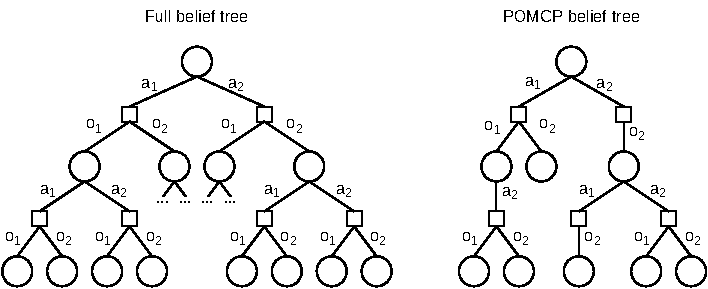
\includegraphics[width=0.8\textwidth]{figures/pomcp_belief_tree.pdf}
    \caption[A full belief tree in contrast with a POMCP belief tree]{Contrasting a full belief tree (left) with a POMCP belief tree (right) for a POMDP with two actions and two observations and a time horizon of two. A belief is stored at every circle node. The full belief tree has 21 belief nodes, while the POMCP belief tree has just nine. The number of nodes of the full belief tree grows exponentially with the time horizon (curse of history), whereas the POMCP belief tree only contains a number trajectories which have been sampled from a generative model. By performing the sampling, the size of the tree is reduced and the curse is \textit{broken}.}
    \label{fig:full_vs_pomcp}
\end{figure}
% TODO: Illustrate belief tree
% See Figure 1 in DESPOT

The key idea of \Gls{pomcp} is to use Monte Carlo sampling both to sample start states from the belief and to sample histories using a generative model \parencite{pomcp}. 

The number of histories to consider in a POMDP grows exponentially with respect to the depth of the planning horizon. This is called the curse of history. POMCP overcomes this limitation by using a generative model to sample state transitions. By doing so, only a subset of histories is considered; the size of the belief tree is reduced and the curse is \textit{broken} (see Figure \ref{fig:full_vs_pomcp}). Furthermore, there is the curse of dimensionality. The belief space has the same dimensionality as the number of states. Thus, the number of beliefs to consider grows exponentially with the number of states. POMCP uses the states encountered during the construction of the tree to represent the belief. Start belief states are sampled from these states, effectively limiting the number of considered belief states and thereby also breaking the second curse. 


% Based on the expected rewards and number of visits of certain actions in the tree, the \glsentryfull{ucb1} algorithm is employed to decide the ratio between exploration and exploitation.

POMCP constructs a search tree representing histories $h$ of actions and observations. At each node, $N(h)$ stores the number of times the node and thereby the coresponding history $h$ has been visited during the sampled trajectories simulated with the generative model. $V(ha)$ gives the action node's expected value that is approximated by the average return of simulations starting at history $h$ and performing action $a$. At every observation node, the belief over the states is maintained by employing a particle filter. Each observation node stores a collection of all states that led to the represented observation during planning. Whenever an observation occurs, the corresponding state is stored in this collection. The states in the collection are called particles and together the particles represent the agent's belief B(h) at the corresponding observation node. The more likely a belief state is, the more often it occurs as a particle in the belief. By using the particle filter method, expensive belief update calculations are not necessary. The collection of states alone aproximates the posterior probability distribution for the belief.

\begin{figure}[htbp]
    \centerfloat
    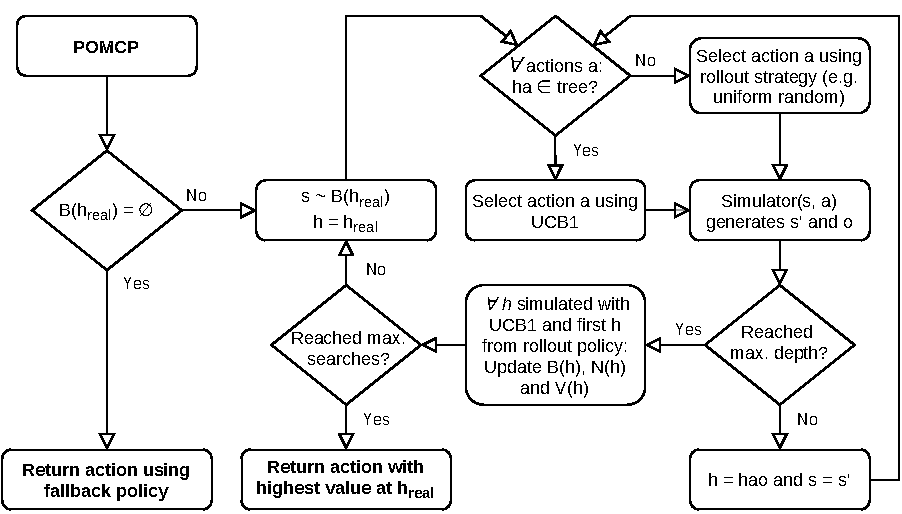
\includegraphics[width=1.034\textwidth]{figures/POMCP.pdf}
    \caption{Flow chart illustrating the \glsentryfull{pomcp} algorithm}
    \label{fig:pomcp}
\end{figure}

Figure \ref{fig:pomcp} illustrates the process of POMCP. The algorithm starts with an initial belief about the environment. If the belief for the current history $h_{real}$ does not contain particles in the beginning of a planning episode, the agent has lost track of the environment's state completely. One could construct a new belief by sampling the state space in this case. However, for the car driving scenario, this approach is too inaccurate. Accessing the real state of the environment to build the belief would be cheating. Instead, we consider the planner to have failed and select actions randomly from this point on.

To select which action to perform in the real environment, a fixed number of forward searches is performed from the current history (often a certain maximum planning time is used alternatively). During these searches using the generative model, the belief and the expected action values are updated. After all searches are complete, the action $a_{best}$ with the highest value at the current history $h_{real}$ is returned. After this action is executed in the real environment, with an observation $o_{last}$ the tree can be pruned. Only the nodes from history $h_{real}a_{best}o_{last}$ onward stay relevant as all other histories are rendered impossible. Then, the process repeats from the new history.

The start state for each search is sampled from the belief at the curret history. The search tree is searched in two stages: Simulation and rollout. As long as the search tree contains child nodes for all actions at the currently considered history, the simulation stage is active. During the simulation stage, no new nodes are added to the tree. The tree is searched using the \glsentryfull{ucb1} algorithm to select actions \parencite{ucb1}. UCB1 chooses actions by the principle of optimism in the face of uncertainty. Even with just little knowledge, the algorithm selects the best action greedily. If this optimistic guess turns out to be correct, the algorithm can further continue to exploit this action and regret is kept to a minimum. If the action leads to a bad return, its value is assumed to deteriorate quickly, allowing the algorithm to select an alternative action. Exploration is controled by enhancing the value of rarely-tried actions with a fixed exploration bonus. State transitions are simulated using the generative model. Given the current history and chosen action, the generative model returns a successive state $s'$, observation $o$, and reward $r$. The successive state $s'$ is then added to the belief at the observation node corresponding to $o$ and the count for the current history is incremented. The search continues from $s'$ in the same manner. If any history is visited for the first time during the simulation stage, the algorithm continues in the rollout stage. First, all action nodes are initialized with initial counts an values. These are usually 0, unless preferred actions are used (See Section \ref{sec:preferred_actions}). Then, the history is \textit{rolled out} further using uniform random action selection and the generative model. The process is continually repeated using the succeeding states from the generative model until a maximum depth is reached in the tree. During the rollout, no further nodes than the ones just initialized are added to the tree. The tree's growth is thereby limited to one level of depth per search. The main purpose of the rollout is to form a first estimation of the newly encountered history. After every search, the values at all nodes encoutered during the search are updated by backpropagating the rewards through the tree.

\subsection{Action and observation space discretization}
\label{sec:discretization}

POMCP is not intended to be used to solve continuous POMDP. However, using POMCP with a continuous states is possible as the particle filter approach can still provide a good approximation of the belief as long as the number of samples is large enough. To account for continuous action and observation spaces, discretization is necessary. Figure \ref{fig:pomcp_cont} shows how POMCP behaves when tasked with solving POMDP with continuous observation or acrtion spaces. If the observations are continuous, the search tree cannot extend beyond the first observation layer as most likely, every observation is unique and thus, no history will ever be visited twice. In the case of continuous actions, the chance of exectuing the same exact action twice is very low. Therefore, in this case likewise no history is reached twice. Planning becomes impossible. However, POMCP can be successfully applied with continuous POMDP by discretizing the action and observation spaces \parencite{pomcp_continuous}.

\begin{figure}[htbp]
    \centering
    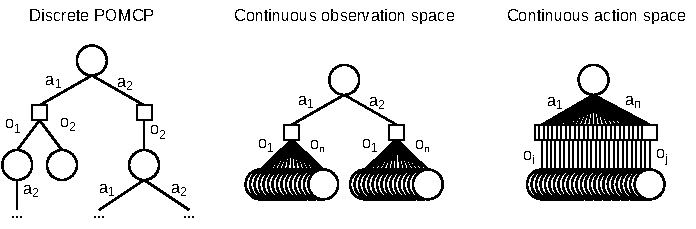
\includegraphics[width=1.0\textwidth]{figures/pomcp_continuous.pdf}
    \caption[Comparison of POMCP belief trees with discrete observations and continuous observations]{Comparison of POMCP belief trees with discrete observations (left) and continuous observations (right) with two actions.}
    \label{fig:pomcp_cont}
\end{figure}

The action space is discretized as outlined before in Section \ref{sec:actions} and the discretization of the observation space is defined in Section \ref{sec:observations}. A balanced discretization resolution is chosen empirically. A too fine grained discretization leads to very wide belief trees and can thereby hinder convergence, while a coarse discretization increases the convergence probability but comes with a lower precision in planning.


% TODO: Add actions and observations tables

\subsection{Particle deprivation and particle injection}
\label{sec:particle_deprivation}

Particle filter approaches, POMCP included, can fail due to a phenomenon called particle deprivation. Because of the random nature of the process, the belief can sometimes converge towards a state that is far from the environment's true state. Particles that differ from the converged state have a low probability to be selected while sampling (low relative count). Hence, with each iteration, they become scarcer until they are completely erased from the belief. At this point, the agent is sure to be in an erroreous state and cannot recover anymore. Particle injection (also called particle reinvigoration) is a method to counteract this problem by introducing a number of random particles to the belief at each iteration \parencite{decision_making_book}. While this reduces the accuracy of the belief, it prevents its complete convergence towards a wrong state. 

Particle injection is used to increase the variance of the belief about the driver model state. Only observable information is used. Concretely, particle injection is implemented by adding driver model states with a random number of remaining actions and the same action as the one that was last observed. The number of remaining actions can be lower than the minimum defined in Section~\ref{sec:driver_model} because this limit is only intended for initial sampling and the true remaining number of driver actions in a particular state might be lower after having performed actions already. Like in the original POMCP paper, the amount of transformed particles that are added before each planning step is $1/16$ of the number of searches. The particles can be added during policy execution, and therefore, do not influence planning time.

% Use term posterior probability distribution? We can only add particles after making an observation so that we can verify that the potential particles to add match this belief.


\subsection{Preferred actions}
\label{sec:preferred_actions}

% TODO: Just say the agent does not act anymore when losing track with the belief instead of using uniformly random action selection? Makes more sense.

% This is strongly related to the particle deprivation problem described in Section~\ref{sec:particle_deprivation}. When the driver is in a distracted or attentive state, any number of remaining actions in this state below the maximum number (see Section~\ref{sec:driver_model}) could be valid and can therefore be part of the driver model states in the belief. In successive iterations, particles that represent drivers switching their state earlier than the true driver, and therefore change their steering behavior, are ruled out and removed from the belief. Thereby, after some iterations, driver model states that have the same or more remaining actions than the true state dominate the belief.

% preferred actions = domain knowledge

\subsection{Generative model}
\label{sec:gen_model}

